\documentclass[12px, a4paper]{article}
\usepackage[utf8]{inputenc}
% ~~~~~~~~~~~~~~~~~~~~~~~~~~~~~~~~~~~~~~~~~~~~~~~~~~~~~~~~~~~~~~~~~~~~~~~~~~~~~~
% Packages to be loaded before others
% ~~~~~~~~~~~~~~~~~~~~~~~~~~~~~~~~~~~~~~~~~~~~~~~~~~~~~~~~~~~~~~~~~~~~~~~~~~~~~~
%%% Packages for LaTeX - programming
%
% Define commands that don't eat spaces.
\usepackage{xspace}
% IfThenElse
\usepackage{ifthen}
%%% Doc: ftp://tug.ctan.org/pub/tex-archive/macros/latex/contrib/oberdiek/ifpdf.sty
% command for testing for pdf-creation
\usepackage{ifpdf} %\ifpdf \else \fi

%%% Internal Commands: ----------------------------------------------
\makeatletter
%
\providecommand{\IfPackageLoaded}[2]{\@ifpackageloaded{#1}{#2}{}}
\providecommand{\IfPackageNotLoaded}[2]{\@ifpackageloaded{#1}{}{#2}}
\providecommand{\IfElsePackageLoaded}[3]{\@ifpackageloaded{#1}{#2}{#3}}

\providecommand{\IfDefined}[2]{%
    \ifcsname #1\endcsname
    #2 %
    \else
    % do nothing
    \fi
}

\providecommand{\IfElseDefined}[3]{%
    \ifcsname #1\endcsname
    #2 %
    \else
    #3 %
    \fi
}
% Calculation with LaTeX
\usepackage{calc}
% Language setting
\usepackage[ngerman]{babel}
% Colors
\usepackage{xcolor}
% Graphics
\usepackage{graphicx}



% ~~~~~~~~~~~~~~~~~~~~~~~~~~~~~~~~~~~~~~~~~~~~~~~~~~~~~~~~~~~~~~~~~~~~~~~~~~~~~~
% Fonts
% ~~~~~~~~~~~~~~~~~~~~~~~~~~~~~~~~~~~~~~~~~~~~~~~~~~~~~~~~~~~~~~~~~~~~~~~~~~~~~~
\usepackage[T1]{fontenc}
% Additional Symbols (Text Companion font extension)
\usepackage{textcomp}



% ~~~~~~~~~~~~~~~~~~~~~~~~~~~~~~~~~~~~~~~~~~~~~~~~~~~~~~~~~~~~~~~~~~~~~~~~~~~~~~
% Math
% ~~~~~~~~~~~~~~~~~~~~~~~~~~~~~~~~~~~~~~~~~~~~~~~~~~~~~~~~~~~~~~~~~~~~~~~~~~~~~~
\usepackage{amsmath}



% ~~~~~~~~~~~~~~~~~~~~~~~~~~~~~~~~~~~~~~~~~~~~~~~~~~~~~~~~~~~~~~~~~~~~~~~~~~~~~~
% Symbols
% ~~~~~~~~~~~~~~~~~~~~~~~~~~~~~~~~~~~~~~~~~~~~~~~~~~~~~~~~~~~~~~~~~~~~~~~~~~~~~~
%%% for Math
%\usepackage{mathrsfs} %% Schreibschriftbuchstaben für den Mathematiksatz (nur Großbuchstaben)
%\usepackage{dsfont}   %% Double Stroke Fonts
%\usepackage[mathcal]{euscript} %% adds euler mathcal font
\usepackage{amssymb}
%\usepackage[Symbolsmallscale]{upgreek} % upright symbols from euler package [Euler] or Adobe Symbols [Symbol]
%\usepackage[upmu]{gensymb}             % Option upmu
%%% common
%\usepackage{wasysym}  %% Doc: http://www.ctan.org/tex-archive/macros/latex/contrib/wasysym/wasysym.pdf
%\usepackage{marvosym} %% Symbols from marvosym Font
%\usepackage{pifont}   %% ZapfDingbats



% ~~~~~~~~~~~~~~~~~~~~~~~~~~~~~~~~~~~~~~~~~~~~~~~~~~~~~~~~~~~~~~~~~~~~~~~~~~~~~~
% Text
% ~~~~~~~~~~~~~~~~~~~~~~~~~~~~~~~~~~~~~~~~~~~~~~~~~~~~~~~~~~~~~~~~~~~~~~~~~~~~~~
%%% Refs
\usepackage[ngerman]{varioref}
\usepackage{hyperref}
%%% Columns
\usepackage{multicol}



% ~~~~~~~~~~~~~~~~~~~~~~~~~~~~~~~~~~~~~~~~~~~~~~~~~~~~~~~~~~~~~~~~~~~~~~~~~~~~~~
% Graphics
% ~~~~~~~~~~~~~~~~~~~~~~~~~~~~~~~~~~~~~~~~~~~~~~~~~~~~~~~~~~~~~~~~~~~~~~~~~~~~~~
\usepackage[all]{xy}
\usepackage{float}
\usepackage{tikz}
%%% Doc: ftp://tug.ctan.org/pub/tex-archive/macros/latex/contrib/subfig/subfig.pdf
% Incompatible: loads package capt-of. Loading of 'capt-of' afterwards will fail therefor
\usepackage{subfig}



% ~~~~~~~~~~~~~~~~~~~~~~~~~~~~~~~~~~~~~~~~~~~~~~~~~~~~~~~~~~~~~~~~~~~~~~~~~~~~~~
% Captions & Style
% ~~~~~~~~~~~~~~~~~~~~~~~~~~~~~~~~~~~~~~~~~~~~~~~~~~~~~~~~~~~~~~~~~~~~~~~~~~~~~~
%%% Doc: ftp://tug.ctan.org/pub/tex-archive/macros/latex/contrib/caption/caption.pdf
\usepackage{caption}
% Aussehen der Captions fuer subfigures (subfig-Paket)
\IfPackageLoaded{subfig}{
    \captionsetup[subfloat]{%
        margin = 10pt,
        font = {small,rm},
        labelfont = {small,bf},
        format = plain, % oder 'hang'
        indention = 0em,  % Einruecken der Beschriftung
        labelsep = space, %period, space, quad, newline
        justification = RaggedRight, % justified, centering
        singlelinecheck = true, % false (true=bei einer Zeile immer zentrieren)
        position = bottom, %top
        labelformat = parens % simple, empty % Wie die Bezeichnung gesetzt wird
    }
}



% ~~~~~~~~~~~~~~~~~~~~~~~~~~~~~~~~~~~~~~~~~~~~~~~~~~~~~~~~~~~~~~~~~~~~~~~~~~~~~~
% Misc
% ~~~~~~~~~~~~~~~~~~~~~~~~~~~~~~~~~~~~~~~~~~~~~~~~~~~~~~~~~~~~~~~~~~~~~~~~~~~~~~
% Theorems
\usepackage{amsthm}
\newtheorem{Definition}{Definition}
\newtheorem{Beispiel}{Beispiel}
\newtheorem{Satz}{Satz}
\newtheorem{Bemerkung}{Bemerkung}
\newtheorem{Algorithmus}{Algorithmus}
\newtheorem{Lemma}{Lemma}
% Listings
\usepackage{listings}
\definecolor{Brown}{cmyk}{0,0.81,1,0.60}
\definecolor{OliveGreen}{cmyk}{0.64,0,0.95,0.40}
\definecolor{CadetBlue}{cmyk}{0.62,0.57,0.23,0}
\definecolor{lightlightgray}{gray}{0.9}
\lstset{
    language=C,                             % Code langugage
    basicstyle=\rm\ttfamily,                % Code font, Examples: \footnotesize, \ttfamily
    keywordstyle=\color{OliveGreen},        % Keywords font ('*' = uppercase)
    commentstyle=\color{gray},              % Comments font
    numbers=left,                           % Line nums position
    numberstyle=\tiny,                      % Line-numbers fonts
    stepnumber=1,                           % Step between two line-numbers
    numbersep=5pt,                          % How far are line-numbers from code
    backgroundcolor=\color{lightlightgray}, % Choose background color
    frame=none,                             % A frame around the code
    tabsize=2,                              % Default tab size
    captionpos=b,                           % Caption-position = bottom
    breaklines=true,                        % Automatic line breaking?
    breakatwhitespace=false,                % Automatic breaks only at whitespace?
    showspaces=false,                       % Dont make spaces visible
    showtabs=false,                         % Dont make tabls visible
    %columns=flexible,                       % Column format
    %morekeywords={someword, otherword},     % specific keywords
}

\usepackage{amsmath}
\usepackage{hyperref}
\usepackage{float}
\usepackage{algorithm}
\usepackage{arevmath}     % For math symbols
\usepackage[noend]{algpseudocode}

\begin{document}
\setlength{\parindent}{0em}
%front
\title{ Stochastik}
\author{Dr. Johannes Riesterer}
\date{\today}
\maketitle\thispagestyle{empty}
 \begin{figure}[H]
    \centering
    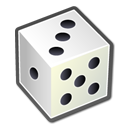
\includegraphics[width=1.0 \textwidth]{images/cover.png}
    \label{fig:diffus}
\end{figure}
\newpage 
\begin{center}
\large
 \copyright Johannes Riesterer \\
\end{center}
\thispagestyle{empty}
\newpage

\section*{Vorwort}
Kann jeder Mathematik lernen? Als Antwort auf diese Frage möchte ich auf den interessanten Lebenslauf
einer der bedeutendsten Mathematikerinnen aller Zeiten eingehen  (Auszug aus Wikipedia):

Emmy Noether war eine deutsche Mathematikerin, die grundlegende Beiträge zur abstrakten Algebra und zur theoretischen Physik lieferte. Insbesondere hat Noether die Theorie der Ringe, Körper und Algebren revolutioniert. Das nach ihr benannte Noether-Theorem gibt die Verbindung zwischen Symmetrien von physikalischen Naturgesetzen und Erhaltungsgrößen an. 

Sie zeigte in mathematischer Richtung keine besondere Frühreife, sondern hatte in ihrer Jugend Interesse an Musik und Tanzen. Sie besuchte die Städtische Höhere Töchterschule – das heutige Marie-Therese-Gymnasium – in der Schillerstraße in Erlangen. Mathematik wurde dort nicht intensiv gelehrt. Im April 1900 legte sie die Staatsprüfung zur Lehrerin der englischen und französischen Sprache an Mädchenschulen in Ansbach ab. 1903 holte sie in Nürnberg die externe Abiturprüfung am Königlichen Realgymnasium – dem heutigen Willstätter-Gymnasium – nach. 


\newpage

%Einfügen des Inhaltsverzeichnisses
\tableofcontents
\newpage
\thispagestyle{empty}
\mbox{}\thispagestyle{empty}
\newpage
%main

\section{Diskrete Modelle}

\begin{Definition}[Laplace Wahrscheinlichkeit]
Sei $\Omega = \{ \omega_1, \cdots , \omega_n\}$ eine endliche Menge. Für $A \subset \Omega$ definieren wir die Wahrscheinlichkeit durch
\begin{align*}
P(A) : = \frac{\#A}{ \# \Omega} \; . 
\end{align*} 
Die Elemente $ \omega_1, \cdots , \omega_n \in \Omega$ nennen wir Elementarereignisse und Teilmengen $A \subset \Omega$ Ereignisse. Die Abbildung
\begin{align*}
P : \mathcal{P} (\Omega) \to [0,1]  
\end{align*}  
nennen wir die Laplace-Verteilung bzw. Gleichverteilung auf $\Omega$.
\end{Definition}


\begin{Definition}[Permutationen und Kombinationen]

\begin{itemize}
\item $Perm_k^n(\Omega, m.W.) : = \{ \omega_1, \ldots, \omega_k \in \Omega^k \}$  Menge aller Permutationen mit Wiederholung.
\item $Perm_k^n(\Omega, o.W.) : = \{ \omega_1, \ldots, \omega_k \in \Omega^k  | \omega_i \neq \omega_j\}$  Menge aller Permutationen ohne Wiederholung.
\item $Kom_k^n(\Omega, m.W.) : = \{ \omega_{i_1}, \ldots, \omega_{i_k} \in \Omega^k  | 1  \leq i_1 \leq  \ldots  \leq i_k \}$  Menge aller Kombinationen  mit Wiederholung.
\item $Kom_k^n(\Omega, o.W.) : = \{ \omega_{i_1}, \ldots, \omega_{i_k} \in \Omega^k  | 1 \leq i_1  \leq \ldots \leq i_k ;  \omega_{i_i} \neq \omega_{i_j} \}$  Menge aller Kombinationen  ohne  Wiederholung.
\end{itemize}
\end{Definition}

\begin{Lemma}
\begin{itemize}
\item $\# Perm_k^n(\Omega, m.W.)  = n^k = \underbrace{n \cdot n \cdots n}_{\text{k-mal}}$
\item $\# Perm_k^n(\Omega, o.W.)  = n_k = n \cdot (n-1) \cdots  (n-(k-1)) = \frac{n!}{(n-k)!}$  
\item $\#Kom_k^n(\Omega, o.W.) = \binom{n}{k} = \frac{n!}{k! (n-k)!}$  
\item $\#Kom_k^n(\Omega, m.W.)  = \binom{n + k -1}{k}$  
\end{itemize}
\end{Lemma}
\begin{proof}
\end{proof}


\begin{Definition}{Diskrete Wahrscheinlichkeitsverteilung}
Es sei $\Omega$ eine (nicht leere) albzählbare Menge. Eine Abbildung 
$P :\mathcal{P}(\Omega) \to [0,1]$ heißt diskrete Wahrscheinlichkeitsverteilung (Wahrscheinlichkeismaß), falls gilt:
\begin{align*}
& P(\Omega) = 1\\
& P \Biggl( \bigcup_{n=1}^{\infty} A_n \biggr)= \sum_{n=1}^{\infty} P(A_n), \text{ mit } A_i \cap A_j = \emptyset \text{ für } i \neq j 
\end{align*}
\end{Definition}


\begin{Beispiel}{Beispiel: Laplace Wahrscheinlichkeit}
$\Omega$ endlich und $P(A) = \frac{\#A}{\#\Omega}$.
 \end{Beispiel}


\begin{Definition}{Bedingte  Wahrscheinlichkeit}
Für $A,B \subset \mathcal{P}(\Omega)$ und $P(B) > 0$ heißt
\begin{align*}
& P(A \; | \;  B) = \frac{P(A \cap B)}{P(B)} \\
\end{align*}
die bedingte Wahrscheinlichkeit (von $A$ unter $B$).
\end{Definition}


\begin{figure}[htp]
      \centering
    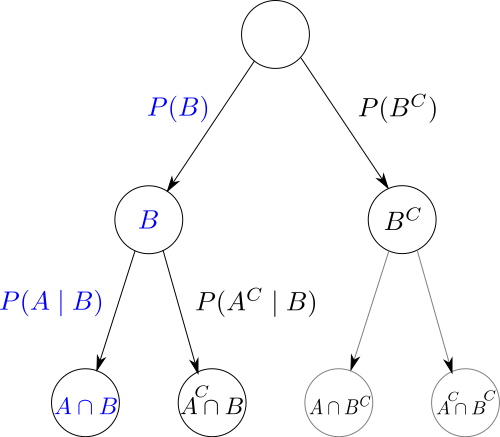
\includegraphics[width=0.5\textwidth]{images/Probability_tree}

      \caption{Quelle: Wikipedia}
\end{figure}



\begin{Satz}{Satz der totalen Wahrscheinlichkeit}
Für eine Zerlegung  $\Omega = \bigcup_{j=1}^{n} B_j, \text{ mit } B_i \cap B_k = \emptyset \text{ für } i \neq k $
\begin{align*}
& P(A ) = \sum_{j=1}^{n}  P(A \; | \;  B_j) \cdot P(B_j)
\end{align*}
\end{Satz}
\begin{proof}
$A = A \cap B \cup A \cap \bar{B}$ und  $A \cap B \cap A \cap \bar{B} = \emptyset$. 
\begin{align*}
& P(A) =  P(A \cap B) + P(A \cap \bar{B}) = P(B) \cdot P(A  \; | \; B) + P(\bar{B}) \cdot P(A  \; | \; \bar{B}) 
\end{align*}
\end{proof}

\begin{Satz}{Satz von Bayes}
Für $A,B \subset \mathcal{P}(\Omega)$ mit  $P(B) > 0$ gilt
\begin{align*}
& P(A \; | \;  B) = \frac{P(B \; | \; A) \cdot P(A)} {P(B)} \\
\end{align*}
\end{Satz}

\begin{proof}
\begin{align*}
& P(A \; | \;  B) =\frac{P(A \cap B)}{P(B)} = \frac{ \frac{P(A \cap B) \cdot P(A)}{P(A)}}{P(B)}  =  \frac{P(B \; | \; A) \cdot P(A)} {P(B)} 
\end{align*}
\end{proof}


\begin{Definition}{Stochastische Unabhängigkeit}
Zwei Ereignisse $A,B$ heißen stochastisch Unabhängig, falls
\begin{align*}
P(A \cap B) = P(A) \cdot P(B)
\end{align*}
gilt.  Somit ist auch $P(A | B) = P(A)$ und $P(B  | A) = P(B)$.
\end{Definition}


\subsection{Naiver Bayes'scher Spam Filter}
Gegeben ist eine E-Mail $E$.  Wir möchten anhand des Vorkommens bestimmter Wörter $A_1, \ldots A_n$ in der Mail entscheiden, ob es sich um eine erwünschte Mail $H$ oder eine unerwünschte Mail $S$ (Ham or Spam) handelt. 
(Typische Wörter wären zum Beispiel "reichwerden",  "onlinecasino" ...)
Aus einer Datenbank kann man das Vorkommen dieser Wörter in Spam und Ham Mails zählen und damit empirisch die Wahrscheinlichkeiten $P(A_i | S)$ und $P(A_i | H) $ des Vorkommens dieser Wörter in Spam und Ham Mails ermitteln.  Wir gehen davon aus, dass es sich bei der Mail  prinzipiell mit  Wahrscheinlichkeit $P(E= S) = P(E= H)= \frac{1}{2}$  um eine erwünschte  Mail $H$ oder eine unerwünschte Mail $S$  handeln kann. 




 Wir machen zudem die (naive) Annahme, dass das Vorkommen der Wörter  stochastisch unabhängig ist, also 
\begin{align*}
P(A_1 \cap \cdots \cap A_n | S) = P(A_1 | S) \cdots P(A_n | S) \\
P(A_1 \cap \cdots \cap A_n | H) = P(A_1 | H) \cdots P(A_n | H)
\end{align*}
gilt.


Mit der Formel von Bayes und der totalen Wahrscheinlichkeit  können wir somit berechnen
\begin{align*}
& P(E=S |  A_1 \cap \cdots \cap A_n) = \frac{P(A_1 \cap \cdots \cap A_n | S) \cdot P(S)}{P(A_1 \cap \cdots \cap A_n)} \\
&=  \frac{P(A_1 | S) \cdots P(A_n | S) \cdot P(S)}{P(A_1 \cap \cdots \cap A_n | H) + P(A_1 \cap \cdots \cap A_n | S)} \\
&=  \frac{P(A_1 | S) \cdots P(A_n | S) \cdot P(S)}{P(A_1 | H) \cdots P(A_n | H)  + P(A_1 | S) \cdots P(A_n | S) } \\
\end{align*}
Bemerkung: $P(E=H |  A_1 \cap \cdots \cap A_n) = 1- P(E=S |  A_1 \cap \cdots \cap A_n) $







%back
\newpage
\listoftables{\addcontentsline{toc}{section}{\listtablename}}
\newpage
\listoffigures{\addcontentsline{toc}{section}{\listfigurename}}
\newpage
\IfDefined{printindex}{\printindex}
\IfDefined{printnomenclature}{\printnomenclature[4.5cm]{}}
\end{document}
